\part{फलित ज्योतिष} \label{part:pred}
एक कुन्डली एक पूरा जीवन दर्शाती है। यह जीवन घटना (मुहूरत), व्यक्ति/देश (लग्न) या वर्तमान स्थिती में उत्पन्न हुए प्रश्न (प्रश्न) का हो सकता है। इन तीनों प्रकार की कुन्डलियों को पढने का तरीका लगभग एक जैसा ही है, परन्तु समान नहीं, इसलिए तीनों को अपने खुदके  अनुभाग मिलेंगे। इनमें से सबसे महत्वपूर्ण है लग्न कुन्डली, क्योंकि ज्योतिष सबसे ज्यादा जीने वाले के ही काम आता है।

अभी के लिए हम हमारा ध्यान बस व्यक्तियों पर केन्द्रित करेंगे, ताकि समझने में आसानी हो। 

हर एक आत्मा अपना स्वभाव और कर्म, जो भाग्य, व्यवहार और  विचारधारा के मिलन से बनते हैं, लेकर शरीर में प्रवेश करती है। यह स्वभाव तथा भाग्य दोनों जीवन भर में धीरे-धीरे अनुभवों के साथ बदलते हैं। इस बदलाव के बाद, जीवन के आखरी क्षणों में जिस भी चीज से आत्मा की आसक्ति रह गई, अगला जीवन उसे वैसा ही मिलता है। उसी आसक्ति और न भुगते हुए कर्मों का हल करने सब कुछ शुरुआत से चालु होता है, पर इस बार थोडे अलग स्वभाव और भाग्य के साथ। यही चक्र तब तक चलता रहेगा, जब तक आत्मा खुदको पूरी तरह जान नहीं लेती।

कोई भी शुद्ध वैज्ञानिक आपको साफ-साफ कहेगा, कि जादु जैसी कोई चीज होती ही नहीं है। १०० साल पहले जिन लोगों को  बिजली और प्रकृति के भिन्न करिष्में समझ नहीं आते थे, आज उन करिष्मों को अनुसंधान के द्वारा समझा गया है, और लोगोंने इस ज्ञान के आधार पर अभियन्त्रण जैसे क्षेत्र खडे किए हैं। इसका साफ मतलब है कि अगर किसी चीज को पूरी तरीके से समझा जाए, तो हम उस चीज का हर परिस्थिती में व्यवहार, तथा उसके व्यवहारों का हर परिणाम ढुंढ निकाल सकते है, बगैर उसे उस परिस्थिती में रखे। अभियन्त्रण में \textenglish{Computer simulation} का पूरा क्षेत्र इसी का प्रत्यक्ष प्रमाण देता है।

अभियन्त्रण के अलावा हम लोगों के व्यवहार में भी यह देख सकते हैं। दो सच्चे दोस्त, जो एक दूसरे को अच्छे से जानते हो, एक दूसरे का हर परिस्थिती में व्यवहार कैसा होगा इसका अनुमान लगा सकते हैं। परन्तु एक व्यक्ति का सब कुछ जानना एक अति जटिल कार्य है, क्योंकि हर कोई समय के साथ धीरे-धीरे बदलता है, और लोग इतने साधारण कभी नहीं होते जितने वे दूसरों को दिखाते हैं, चाहे कोई कितना भी पास का क्यों न हो। इसी कारण हम हमारी बुद्धि से इस जगत् के बदलावों का पूरी तरह अनुमान नहीं लगा सकते। यह सीमा सर्व-व्यापी परमात्मा, जो हर जीव का आधार है, उसपर लागू नहीं होती।

भगवद्गीता में श्री कृष्ण कहते हैं कि वे सबके बारे में सब जानते हैं, पर कोई उनके बारे में कुछ नहीं जानता। इसका दूसरा मतलब है कि आकाश में चलने वाले ज्योतियाँ, जिनको वही चलाते हैं, उनमें जगत् में पाए जाने वाले हर सम्भव स्थिती, हर सम्भव प्रश्न के बारे में हमेशा सटीक जानकारी रहेगी। इसी कारण फलित ज्योतिष को ``वेदचक्षु'' भी कहा जाता है, क्योंकि उसके द्वारा वेदों के अनमोल ज्ञान को प्रत्यक्ष देखा जा सकता है।

जो आत्माएँ  खुदको जितना ज्यादा गुणों में मानते हैं, और विभिन्न चीजों में आसक्ति रखते हैं, उनपर इस प्रणाली की भविष्यवाणियाँ अत्यंत सटीक रूप से काम करती हैं। परन्तु यदि व्यक्ति आध्यात्म के मार्ग पर लगा हो, या अपने निर्णयों को और खुदको कोशिश करके बदल रहा हो, तब  वह प्रणाली में लिखे हुए भविष्य से थोडा परे होगा। क्योंकि बहुत कम लोग  अपने कर्मों और मन के ऊपर सचेत रूप से नियंत्रण रखते हैं, प्रणाली मे लिखी हुई लगभग ८०\% चीजे निश्चित रूप से देखने को मिलती हैं।

जैसे पहले कहा गया है, हर एक आत्मा का अपना भाग्य, व्यवहार और विचारधारा होते हैं, जो प्रणाली में अलग देखने मिलेंगे। इनमें से भाग्य को कुछ भी करके बदला \bt{नहीं} जा सकता, और वह भुगतना ही पडता है। परन्तु व्यक्ति के प्रयास से विचारधारा तथा व्यवहार बदले जा सकते हैं, जिससे भविष्य का भाग्य लिखा जाता है। इसका दूसरा अर्थ यह भी हुआ कि आत्मा अपना भाग्य खुद लिखती है, और हर एक दुख और खुशी, जो उसे उसके मार्ग पर मिलती है, वह उसका अपना कमाया हुआ पुरस्कार है। 

प्रणाली में सारे नियम एकदम साफ हैं,  हर कर्म के परिणाम के साथ। चाहे कोई कुछ भी मानें या न मानें, सब कुछ नियम के अनुसार ही होगा। सत्य को अस्वीकार करके उससे भागा नहीं जा सकता।
\chapter[व्यक्ति]{लग्न/राशी कुन्डली} \label{chap:lagna}
लग्न कुन्डली जन्म के समय बनाई जाती है, तथा एक व्यक्ति के जन्म तक के उसके भाग्य, व्यवहार तथा विचारधारा की जानकारी रखती है। जो लोग खुदको सचेत रूप से बदलते हैं, उनकी लग्न कुन्डली सालों के बीतने पर असटीक होना शुरू होती है। ऐसे स्थिती में लग्न न उपयोग करके प्रश्न कुन्डली ज्यादा फायदेमन्द रहेगी, उसी प्रकार जैसे आप बिमार होने पर डॉक्टर को सालों पुराना रिपोर्ट नहीं दिखाएंगे। परन्तु स्वभाव इतने जल्दी नहीं बदलते, इसलिए ५०\% चीजें ऐसे सचेत व्यक्ति में भी लग्न कुन्डली से सही आ ही जाते हैं।

कुन्डली को दर्शाने के दो मुख्य तरीके हैं -
\begin{enumerate}
    \item \bt{उत्तर भारतीय} : घर स्थिर, राशियाँ स्थानान्तरित
    \item \bt{दक्षिण भारतीय} : घर स्थानान्तरित, राशियाँ स्थिर
\end{enumerate}
जैसे कि देखा जा सकता है, दोनों प्रतिनिधित्वों में कोई फर्क नहीं हैं, दोनों उसी सत्य को बस अलग दिशा से देखते हैं। कौनसा बहतर है इस मतभेद में न जाते हुए इस पुस्तक में बस उत्तर भारतीय प्रणाली का उपयोग किया गया है। जिसे दक्षिण भारतीय प्रणाली मे रूची हो, वह अपने हिसाब से राशियों को स्थिर करके घर घुमा सकता है: अंत मे परिणामों में कोई फर्क नहीं आएगा।

एक उत्तर भारतीय कुन्डली ग्रहों के बिना \autoref{fig:grundkarte} में दर्शायी गई है। आकडे राशियाँ हैं, जो \autoref{fig:grundkarte} के लिए मूल घर क्रमांक भी दिखाते हैं। यह मूल घर क्रमांक हमेशा वही रहेंगे, परन्तु राशी चक्र घुम सकता है। जो राशी पहले घर में प्रकट होगी, उसे लग्न राशी कहेंगे, और बाकी घरों के राशियों की गिनती इस घर से चालु होगी। \autoref{fig:grundkarte} में लग्न राशी १ है : इस व्यवस्था को कालपुरुष कुन्डली भी कहा जाता है।
\begin{figure}[bth]
    \centering
\begin{tikzpicture}[scale=1.5, line width=0.8pt]
    % Outer square vertices
    \coordinate (A) at (0,0);
    \coordinate (B) at (4,0);
    \coordinate (C) at (4,4);
    \coordinate (D) at (0,4);

    % Midpoints of the outer square's sides
    \coordinate (E) at (2,0);
    \coordinate (F) at (4,2);
    \coordinate (G) at (2,4);
    \coordinate (H) at (0,2);

    % Draw the outer square
    \draw (A) -- (B) -- (C) -- (D) -- cycle;

    % Draw the inner square
    \draw (E) -- (F) -- (G) -- (H) -- cycle;

    % Draw the diagonals of the outer square
    \draw (A) -- (C);
    \draw (B) -- (D);

    % Region labels
    \node at (1,0.5) {६};
    \node at (3,0.5) {८};
    \node at (3.5,1) {९};
    \node at (3.5,3) {११};
    \node at (3,3.5) {१२};
    \node at (1,3.5) {२};
    \node at (0.5,3) {३};
    \node at (0.5,1) {५};
    \node at (2,1) {७};
    \node at (3,2) {१०};
    \node at (2,3) {१};
    \node at (1,2) {४};
\end{tikzpicture}
\caption{कालपुरुष कुन्डली}
\label{fig:grundkarte}
\end{figure}

घर, राशी और ग्रह ज्योतिष्शास्त्र की नीव हैं। हर एक का अपना विशेष स्वभाव होता है, जिसे जो अच्छे से समझ लें, उसे ज्योतिष्शास्त्र ग्रहण करना बहुत आसान हो जाएगा। सारे सूत्र तथा विधियाँ इन्हीं स्वभावों के आधार पर रचे गए हैं, जो देखने में जितने सरल लगते हैं, हैं उतने ही गहरे। इन नीवों पर जितना समय दें उतना कम ही हैं, इसलिए उनकी गहन चर्चा होगी।

क्योंकि यह सारे नीव एक दुसरे से घनिष्ठ रूप से सम्बन्धित  हैं, कई बार बहुत चीजे उनके स्पष्टीकरण से पहले ही प्रकट हो जाएंगी। इसका उपाय एक ही है : इन्हें समझाने वाले तीनों अध्यायों को कम से कम दो-तीन बार क्रम से पढना पडेगा, तब ही सारे संकल्पनाएँ दिमाग में साफ होंगी, और भ्रम दूर हटेंगे। इन पुनरावृत्तियों को सरल बनाने हेतु सबसे आसान क्रम है - \bt{घर-राशी-ग्रह}, जिसके हिसाब से आगे के अध्याय लिखे गए हैं।
\section[घर]{घर (भाव)} \label{sec:haus}
\autoref{fig:grundkarte} में बने हुए हर एक भाग को घर या भाव कहते है। हर एक घर जीवन में पाए जाने वाले एक तरीके के चीजों को दर्शाता है, और उसमें आने वाले ग्रह व राशी उस व्यक्ति (जिसकी कुन्डली बनाई गई है) की उन चीजों के प्रति विचारधारा।
\begin{setdef}
    \bt{घर} - विचारधारा, इच्छा, सामग्री जो मिली हुई है और खुदसे जीवन में चलके आएगी
\end{setdef}
ध्यान रहे कि ज्योतिष्शास्त्र में कुछ भी स्वभावतः अच्छा या खराब नहीं होता --
\begin{example}
मिली हुई सामग्री में पारिवारिक धन आ सकता है, या परिवार में चलते आ रहे शाप भी। 
\end{example}
असल में क्या मिलेगा यह घर की स्थिती और उसका स्वभाव देखकर ही जाना जा सकता है। जिन घरों में जितने ज्यादा ग्रह वास करते है, उनमें उतना ही कम स्वातंत्र्य होता है। खाली घरों में खुद के हिसाब से कर्म करने की सबसे अधिक स्वतंत्रता मिलती है।

घरों के लिए उनके मूल क्रमांक तथा उन्हें गिनने की विधि बहुत महत्वपूर्ण हैं --
\begin{setdef}
    \begin{tabular}{m{15.5cm}}
    \bt{घर गिनती} - एक घर, जिसका मूल क्रमांक $\alpha$ है, उससे $\beta$ घर आगे स्थित घर का मूल क्रमांक $\alpha+\beta-1$ होगा। यदि अंत में पाया  गया क्रमांक १-१२ के आकडों में नहीं  आता है, तो उसमें १२  मिलाए या उससे १२ घटाए, ताकि मूल क्रमांक इस सीमा के अंदर आ सके।\\\hline \bt{उलटी घर गिनती} - एक घर, जिसका मूल क्रमांक $\alpha$ है, उससे $\zeta$ घर पीछे स्थित घर का मूल क्रमांक $\alpha-\zeta+1$ होगा। इस  क्रमांक को भी ऊपर दिए गए तरीके से अंत में १-१२ के बीच लाना होगा।
    \end{tabular}
\end{setdef}
यदि दो मूल क्रमांकों ($\alpha_1, \alpha_2$) के बीच का फर्क ($\beta$) निकालना है, तो ऊपर के सूत्र को उलटा भी लगाया जा सकता है --
\begin{syntax}
    यदि एक घर (मूल क्रमांक $\alpha_1$) से दूसरे घर (मूल क्रमांक $\alpha_2$) तक की दूरी ($\beta$) निकालनी है, तो इसका समीकरण
    \begin{equation}
        \beta = \alpha_2 - \alpha_1 +1
        \label{eq:forcalc}
    \end{equation}
    से दिया जाएगा। सामान्य रूप से $\beta$ को भी १२ मिलाके या घटाके १-१२ की सीमा में लाना चाहिए। उलटे घर गिनती के लिए यही समीकरण
    \begin{equation*}
        \zeta = \alpha_1 - \alpha_2 +1
    \end{equation*}
    का रूप लेगा।
\end{syntax}
उलटी और सीधी घर गिनती के बीच एक बहुत साधारण सम्बन्ध है --
\begin{syntax}
    यदि कोई दो घरों के बीच सीधे और उलटे घर गिनती का सम्बन्ध क्रमशः $\phi$ तथा $\lambda$ है, तो
    \begin{equation*}
    \phi + \lambda = 14
\end{equation*}
हमेशा सत्य है।
\end{syntax} 
यदि किसीको लग रहा हो कि यह सूत्र ऊपर के सूत्र से मिलता नहीं, क्योंकि $\beta+\zeta$ को मिलाकर हमेशा $2$ आ रहा है, तो भ्रमित मत होईए, यह कोई गलती नहीं है। यह खेल है चक्र का, जो एक तो सीधे या फिर उलटे घर गिनती को हमेशा १-१२ की सीमा के बाहर फेंकता है, जिसके कारण उसे सीमा में लाने के लिए उसमें हमेशा १२ जोडना पडता है। इसको ध्यान में रखते हुए देखा जा सकता है कि $12 + 2 = 14$ का आंकडा आ जाएगा। पाठक को प्रोत्साहित किया जाता है, कि इस सूत्र की पुष्टि स्वयं करें, तथा यह क्यों काम करता है उसे अच्छे से समझें।

यह घर गिनती नियम सामान्य दिखते हैं, परन्तु बहुत उपयोगी पडेंगे।

उनसे देखे जा सकने वाले चीजों के स्वभावानुसार, हर घर का अपना अलग प्रभाव होता है, जो जीवन के लिए कभी समर्थक और कभी बाधक बनेगा। यह प्रभाव उनके मूल घर क्रमांक से साथ जुडे होते हैं, और घर गिनती के दौरान प्रकट होंगे।
\begin{setdef}
    एक घर (मूल क्रमांक $\alpha$) से $\beta$ आगे स्थित घर उस घर (मूल क्रमांक $\alpha$) के लिए वैसे ही प्रभाव देगा, जैसे घर क्रमांक $\beta$ लग्न (मूल क्रमांक १) के लिए देता है।
\end{setdef}
इसका मतलब बस इतना है, कि एक $\beta$ क्रमांक आगे वाले घर का  लग्न (मूल क्रमांक १) पर जो प्रभाव  होगा, वैसा ही प्रभाव $\beta$  क्रमांक आगे वाले घर का  हर घर पर तुलनात्मक रूप से  होगा। यह हमेशा सत्य है क्योंकि लग्न से $\beta$ क्रमांक आगे वाले घर का मूल क्रमांक $\beta$ ही होता है। इस प्रकार, कुन्डली को घुमाके बहुत चीजें प्रकाशित हो सकती हैं, जो शायद व्यक्ति से इतने सरल रूप से जुडे न हों।

इस सूत्र का एक और फायदा है कि हर घर क्रमांक के यदि गुण पता हो, ते हर घर के हर तरह के गुण पता हो जाएंगे। ध्यान रहे कि इस सूत्र का  अधिकतम ३ बार उपयोग किया जा सकता है --
\begin{example}
    पर्दादाजी के जीवन के बारे में देखने हम व्यक्ति के पिता के पिता के पिता (९ से ९ से ९) वाला घर लग्न बना सकते हैं, पर उनसे पहले वाली पीढ़ी तक  नहीं पहुँच सकते।
\end{example}
ध्यान रहे कि जितना पीछे जाएंगे, उतनी सटीकता कम होते जाएगी, क्योंकि  कुन्डली मूलतः व्यक्ति की है।

हर घर के आठ समानान्तर कक्ष होते हैं, जिनके मालिक शुरुआत से बढती डिग्री में --
\begin{setdef}
    १ - शनि, २ - गुरू, ३ - मंगल, ४ - सूर्य, ५ - शुक्र, ६ - बुध, ७ - चन्द्र, ८ - लग्न
\end{setdef}
हैं। यह क्रम ग्रहों की उतरती गति को भी दिखाता है। छाया ग्रह नहीं लिए जाएंगे।
\subsection[वर्गीकरण]{घरों के प्रकार} \label{subsec:hausart}
\ut{\autoref{subsec:hausart} से  घर क्रमांक (घ.क्र) का मतलब  मूल घर क्रमांक होगा।}
\begin{itemize}
    \item उपचय घ.क्र - ३, ६, १०, ११ - समय के साथ बढते जाते हैं
    \item केन्द्र घ.क्र - १, ४, ७, १० - जो चीज़ें प्रतिदिन लगती हैं
    \item अंधकार घ.क्र - ६, ७, ८ - जहाँ व्यक्ति सही से देख नहीं सकता
    \item त्रिक् घ.क्र - ६, ८, १२ - सामान्यतः बाधा  डालने वाले। ३ भी परेशान करता है, परन्तु त्रिक् में नहीं गिना जाता
    \item त्रिकोण - \begin{enumerate}
        \item धर्म घ.क्र - १, ५, ९ - आशीर्वाद
        \item अर्थ घ.क्र - २, ६, १० - जीवन के लिए आवश्यक/उपयोगी चीज़ें
        \item काम घ.क्र - ३, ७, ११ - इच्छा/इच्छापूर्ति
        \item मोक्ष घ.क्र - ४, ८, १२ - मनश्शान्ति/त्रृप्ति, अध्यात्म
    \end{enumerate}
\end{itemize}
काम त्रिकोण + घ.क्र[६] का राहु के साथ हमेशा कोई सम्बन्ध रहता है, और यहीं पुनर्जन्म का कारण बनते हैं।
\subsection[घर गुण]{क्रमांकों के स्वभाव} \label{subsec:hauszahlverhalten}
सारे क्रमांकों के मूल स्वभाव क्रम से दिए गए हैं। यह सारे स्वभाव \bt{अपरिवर्तनीय} हैं, और कुन्डली प्रकार पर निर्भर नहीं। बाकी के गुण \composite{मिलावटी} हैं, जो कुन्डली घुमाकर आते हैं।

हर क्रमांक का एक मूल गुण होता है, और सारे बाकी गुणों का किसी तरह इस मूल से सम्बम्ध होगा।
\subsubsection{१ - स्वास्थ्य, जीवन का ढाँचा}
\begin{itemize}
    \item \bt{शरीर} - बुद्धि, सिर, दिमाग, बाल, त्वचा
    \item \bt{पात्र} - स्वयं
    \item व्यक्तित्व (व्यक्ति को जानने वालों को बाहर से दिखने वाला), प्रसिद्धि, अहंकार
\end{itemize}
इस घ.क्र को \autoref{fig:grundkarte} में `लग्न' भी कहा जाता है, तथा इस पहले घर में आने वाली राशी को `लग्न राशी'। इनको `लग्न कुन्डली' से मिश्रित न करें।
\subsubsection{२ - जीवनावश्यक सामग्री}
\begin{itemize}
    \item \bt{शरीर} - चेहरा,  दाँत, मुँह, आँख, जीभ
    \item \bt{पात्र} - पास का परिवार (जिसमें जन्म होता है)
    \item \composite{बचपन}, वाणी, धन
    \item भोजन आदतें, \composite{संस्कार, दूसरा विवाह}, शिक्षा (प्राथमिक)
\end{itemize}
\composite{\bt{जहाँ}} शरीर के दो अंग होते हैं, वहाँ २-६ दायाँ तथा ८-१२  बायाँ (व्यक्ति के दृष्टी से) भाग दर्शाते हैं। दोनो भागों की सामान्य स्थिती के लिए दायाँ घर ही लेंगे। स्त्रियों के लिए यह क्रम उलटा लेंगे।
\subsubsection{३ - संघर्ष}
\begin{itemize}
    \item \bt{शरीर} - नाँक, कान, हाथ, कन्धे, गर्दन, ऊपरका सीना, ऊपरकी पीठ
    \item \bt{पात्र} - छोटे भाई-बहन, समर्थक (दाएँ हाथ जैसे), पड़ोसी
    \item परिश्रम, साहस, इच्छाशक्ति, कौशल, युद्ध, बदलाव
    \item शारिरीक स्वास्थ्य, दस्तावेज़, शस्त्र, सुरक्षा, लक्ष्य
    \item संवाद (किसी भी प्रकार का), शौक, अवचेतन मन, यात्रा (छोटी)
    \item मैथुन, \composite{प्रजनन क्षमता}, यौन अभिमुखता
\end{itemize}
यह क्रमांक मन की शान्ति साधारण रूप से भंग करता है।
\subsubsection{४ - मनश्शान्ति}
\begin{itemize}
    \item \bt{शरीर} - हृदय, फेफड़े, सीना (लडकियों में स्तन भी), पीठ, गर्भ
    \item \bt{पात्र} - माता, निकट मित्र, विस्तारित परिवार, सारे जो व्यक्ति के लिए काम करते हैं
    \item मन, भावना, उपचार, सुख, सुविधा, शुद्धता
    \item सम्पत्ति (व्यक्ति के लिए महत्वपूर्ण सब), गाडी, घर, समाज
    \item मातृभूमी, सुरक्षा (का भाव), शिक्षा (शालेय)
\end{itemize}
\subsubsection{५ - पूर्व पुण्य}
\begin{itemize}
    \item \bt{शरीर} - पाचन, ऊपर की पीठ, छोटी आंतें
    \item \bt{पात्र} - सन्तान (और उनका जन्म), विद्यार्थी, समर्थक (तथा व्यक्ति के साथ चलने वाले)
    \item रचनात्मकता, भविष्य की योजना, जीवन को देखने का दृष्टिकोण
    \item संयम, सहनशक्ति, मन्त्र, सफलता, शिक्षा (स्नातक)
    \item प्रेम सम्बन्ध, त्याग, बुद्धि, पसंद-नापसंद, मनोरंजन
\end{itemize}
इस क्रमांक में व्यक्ति को उत्तरदायित्व उठाना और निभाना पडता है।
\subsubsection{६ - दुर्बलता}
\begin{itemize}
    \item \bt{शरीर} - नीचे की पीठ, नीचे का पेट, बडी आंतें
    \item \bt{पात्र} - नौकर, शत्रु (व्यक्ति को नहीं पसंद ऐसे लोग भी शामिल), पालतु पशु
    \item नौकरी/सेवा, समय-सारिणी, रोग (जीवनशैली के कारण)
    \item उधारी, झगडा, \composite{सम्बन्ध विभाजन}
    \item ब्रह्मचर्य, बाधा, पुनःप्रयत्न, मिलने वाला उपहार
    \item षडरिपु (काम, क्रोध, लोभ, मद्, मोह, मत्सर्य), स्पर्धा भाव
\end{itemize}
\subsubsection{७ - माया / बाहरकी दुनिया}
\begin{itemize}
    \item \bt{शरीर} - रीढ़ की हड्डियाँ, गुर्दे (दोनों), प्रजनन अंग
    \item \bt{पात्र} - जीवनसाथी, साझेदार, खुले शत्रु
    \item विवाह, धंधा, मानव सम्बन्ध
    \item समाज, सामाजिक जीवन, सामाजिक प्रतिष्ठा
    \item यात्रा (घर पीछे छोडकर कहीं जाना), दयालुता (हृदय - जितना तामसिक प्रभाव उतना अधिक दयालु)
    \item इच्छा, संतुलन, पद प्राप्ति, सूर्यास्त
\end{itemize}
इस क्रमांक में स्थित चीजें व्यक्ति को पूर्णता का भाव देती हैं। बस भाव, क्योंकि आत्मा वास्तव में पूर्ण ही होती है।
\subsubsection{८ - रहस्य, अंधेरा, परिवर्तन}
\begin{itemize}
    \item \bt{शरीर} - मलाशय, गुदाद्वार
    \item \bt{पात्र} - \composite{ससुराल}
    \item अनुसंधान, साधना, गूढ़ विद्या, आत्म-चिंतन (आवश्यकता से अधिक), अस्थिरता, अलगाव
    \item अंत (एक जीवन-चरण का, जिससे परिवर्तन), विरासत (व्यक्ति को मिलने वाला), दबाव
    \item निज दोष (खुदकी गलतियों का परिणाम), घोटाला, उधारी (लेने की क्षमता), कर (सारा जो दूसरे को देने हेतु पाया गया)
    \item दीर्घायू, दीर्घकालीन रोग (कर्मों का दन्ड), \composite{दुर्भाग्य}, पतन
    \item समुद्री यात्रा, प्राकृतिक आपदा, \composite{पूर्व जन्म, अगला जन्म}
    \item व्यक्तित्व (भीतर से, जो किसीको दिखता नहीं), मूल (संस्कृति, जिसमें व्यक्ति अपना बचपन बिताता है)
    \item \composite{विवाह का टिके रहना, यौन सम्बन्ध}
\end{itemize}
\subsubsection{९ - धर्म, दीर्घ विद्या}
\begin{itemize}
    \item \bt{शरीर} - जांघें
    \item \bt{पात्र} - पिता, पूर्वज, गुरू, मुख्य (\textenglish{boss/head}), अधीनस्थ (जो व्यक्ति के अधीन काम कर रहे हो)
    \item शिक्षा (स्नातकोत्तर), लंबी यात्रा (मानसिक भी हो सकती है), स्वतंत्रता, धर्म, जीवन सिद्धांत
    \item भाग्य, पूर्व अनुभव, सृजन, दीर्घकालिक योजना
    \item लडकियों के लिए सन्तान जन्म (व्यक्ति का बच्चा पैदा होने के  समय की स्थिती)
\end{itemize}
\subsubsection{१० - कर्म}
\begin{itemize}
    \item \bt{शरीर} - घुटने, \composite{दृष्टी (आंखों की)}
    \item \bt{पात्र} - सारे, जिनके लिए व्यक्ति काम करता/करती है
    \item कार्यक्षेत्र (स्थान तथा कर्म प्रकार), जीवनके सारे कर्म, सार्वजनिक स्तर
    \item दूरदृष्टी, चित्त, एकाग्रता
\end{itemize}
\subsubsection{११ - लाभ}
\begin{itemize}
    \item \bt{शरीर} - घुटने से टखने तक का भाग
    \item \bt{पात्र} - बडे भाई-बहन, मित्र
    \item उत्पन्न, इच्छापूर्ति, \composite{वेतन, सन्तान जन्म}
    \item \composite{दन्ड (कर्मों का)}
\end{itemize}
क्रमांक ११ का दन्ड ८ से थोडा अलग है। ८ के दीर्घकालिक रोग  लंबे समय तक रहते हैं, परन्तु उनके उपाय उपलब्ध होते हैं, जो  बहुत पीड़ा के बाद उनको जीवन से निकाल देंगे, या कम से कम व्यक्ति के लिए पहले से अच्छी स्थिती निर्माण करेंगे। ११(६ से ६) वाले दन्ड का \bt{कोई उपाय नहीं} होता, और उन्हें सिर्फ भुगता जा सकता है। साधारण रूप से ऐसी बिमारियों को कोई सही से पहचान ही नहीं पाता, और वे जैसे आती हैं, वैसे ही दन्ड का समय समाप्त होने पर स्वयं गायब हो जाएँगी।
\subsubsection{१२ - समर्पण}
\begin{itemize}
    \item \bt{शरीर} - टखने से नीचे का पैर
    \item \bt{पात्र} - अलग संस्कृति के लोग (व्यक्ति के लिए), ज्योतिषी, वैद्य
    \item शयन, आराम, आश्रम, \composite{शयनकक्ष, अस्पताल}
    \item यात्रा (अलग संस्कृति के लोगों के बीच / उनसे सम्बन्ध), \composite{अलगाव, यौन सुख}
    \item दान, खर्चा, निवेश (पूँजी लगाना), नुकसान (अंत, जिसके बाद उसी प्रकार का कुछ नया नहीं आता)
    \item बन्धन, मुक्ति/मोक्ष, प्रतिबद्धता, \composite{मृत्यु, भक्ति, मन की कल्पनाएँ, उपवास}
    \item भूतकाल, आशिर्वाद, \composite{पितर}, अलग संस्कृति
\end{itemize}

\section[राशी]{राशी} \label{sec:zeichen}
राशियों में मिलने वाले गुणों और स्वभावों के कई स्त्रोत हैं --
\begin{enumerate}
    \item चिन्ह (महत्वपूर्ण)
    \item राशी मालिक / स्वामी
    \item विभाजन (डिग्री व प्रकार के हिसाब से)
    \item राशी क्रमांक (जैसे \autoref{fig:grundkarte} में देखा जा सकता है)
    \item राशी में उच्च, नीच स्थिती प्राप्त करने वाले ग्रह
    \item कालपुरुष कुन्डली (\autoref{fig:grundkarte}) में जो राशी जिस घर में आती है, उस  घ.क्र का \ut{मूल स्वभाव}
\end{enumerate}
उच्च ग्रह और राशी मालिक के गुण सशक्त, तथा नीच ग्रह के गुण दुर्बल मिलेंगे। राशी चिन्ह के आधार पर राशियों को विभाजित किया जाता है।  हर ऐसे विभाजन के  अलग उपयोग और निष्कर्ष होते हैं, जो ज्यादातर प्रश्न कुन्डली में फायदेमंद लगेंगे, लग्न में नहीं।

किसी कुन्डली में जो राशी जिस घ.क्र में आएगी, उस राशी के गुण उस घ.क्र के स्वभाव (\composite{मिलावटी} भी) पर  आजीवन प्रभाव डालेंगे।  ये प्रभाव व्यक्ति के लिए अच्छे हैं या खराब, इसकी जानकारी घर की स्थिती तथा व्यक्ति का दृष्टिकोण देंगे।
\begin{example}
    \begin{tabular}{c}
लग्न-१२  एक तो अपने संस्कृति से सामान्यतः दूर ही रहेगा, या उसे छोडकर कभी दूर जाएगा ही नहीं। \\\hline उसके टखने के नीचे का पैर एक तो  तगड़ा होगा, या उसी के कारण उसका स्वास्थ्य बिगडते रहेगा।
    \end{tabular}
\end{example}
हर राशी का अपना स्वर  है। व्यक्ति के नाम का पहला स्वर जिस भी राशी का होगा, उस राशी के गुण तथा  उस घ.क्र के गुण, जहाँ यह राशी लग्न कुन्डली में आती है, व्यक्ति के जीवन पर प्रभावशाली रहते हैं। यदि उस घर में और ग्रह हो, तो उनके तथा उनके स्वामित्व घरों के भी गुण इनमें मिश्रित हो जाएँगे। यदि ऐसा घ.क्र  ज्यादा व्यथा में  आ गया तो उसका अंग भाग सताएगा। यदि मालिक  भी व्यथा में आया तो बचपन कठिन जाता है।

राशी गिनती की भी बहुत बार आवश्यकता पडती है, और इसका घर गिनती के साथ सीधा सम्बन्ध है --
\begin{setdef}
    \bt{राशी गिनती} - एक घर, जिसका मूल क्रमांक $\alpha$ है, तथा जिसमें राशी $\delta$ स्थित हो, उससे $\beta$ घर आगे वाले घर में राशी $\delta+\beta-1$ स्थित होगी। यदि अंतिम आकडा १-१२ के बीच न हो, तो उसमें १२ मिलाए, या उससे १२ घटाए, ताकि राशी क्रमांक इस सीमा में आ सके।
\end{setdef}
जैसे की साफ हो चुका होगा, इन दोनों गिन्तियों में कोई फर्क नहीं है। दो राशियों के बीच का क्रमांक फर्क भी \autoref{eq:forcalc} के हिसाब से निकाला जा सकता है।
\subsection[वर्गीकरण]{राशियों के प्रकार} \label{subsec:zeichenart}
सारी राशियाँ उनके चिन्ह के आधार पर बाँटी गई हैं। ध्यान दें, कि सारे निम्नलिखित विभाजन बस राशीयों की प्रकृति को बाँटते हैं -- इनसे विचलित होने की कोई आवश्यकता नहीं।
\begin{itemize}
    \item गुण - जो ग्रह जैसे राशी में आते है, उनका व्यवहार वैसा बनता है \begin{itemize}
        \item \bt{\rajas{चल}} - १, ४, ७, १० - यह राशियाँ समय के प्रवाह में भूतकाल छोड देगी, व बदलाव पसंद करती हैं
        \item \bt{\tamas{स्थिर}} - २, ५, ८, ११ - यह राशियाँ कभी भूतकाल भूलती नहीं और अडी रहती हैं
        \item \bt{\satva{द्विस्वभाव}} - ३, ६, ९, १२ - पहले १५डि स्थिर और बादके १५डि चल जैसा व्यवहार। व्यक्ति यहाँ काफी उलझन में रहता है, और बहुत सोच-विचार के बाद ही निर्णय ले पाएगा
    \end{itemize}
    \item उदय \begin{itemize}
        \item \bt{शीर्षोदय} - ३, ५, ६, ७, ८, ११ - सफलता आसान
        \item \bt{पृष्ठोदय} - १, २, ४, ९, १० - सफलता मुश्किल, असफलता
        \item \bt{उभ्योदय} - १२ - दोनों स्वभाव सम्भव
    \end{itemize}
    \item गीलापन  - जितना सूखा उतना ज्यादा प्रयास आवश्यक, व उन अंगों में खून के कमी से रोग हो सकते हैं \begin{itemize}
        \item \bt{पानी में निवासी} - ४, ८, १०, १२
        \item \bt{गीले} - २, ३, ६, ११
        \item \bt{सूखे} - १, ५, ७, ९
    \end{itemize}
    \item काल - सूर्योदय से दो घंटे राशी ५ के होते हैं। उसके बादके दो घंटे ६ के। ऐसा चलता रहेगा जब तक अगला दिन नहीं चालु होता।
    \item अंतर - वैदिक ज्योतिष में हम मानते है कि सारे चिन्द समानान्तर (डिग्री के हिसाब से) हैं, परन्तु यह वास्तव में सत्य नहीं \begin{itemize}
        \item \bt{लंबे} - ५, ६, ७, ८
        \item \bt{मध्य} - ३, ४, ९, १०
        \item \bt{छोटे} - १, २, ११, १२
    \end{itemize}
    \item पैरों की संख्या। मानिए कि $\gamma$  १५डि है \begin{itemize}
        \item \bt{चतुष्पद} - १, २, ५, ९ ($\gamma, 30$), १० ($0,\gamma$) - शारिरीक बल। कर्म पर ज्यादा ध्यान
        \item \bt{द्विपद} - ३, ६, ७, ११ - बौद्धिक बल। सोच-विचार में ज्यादा ध्यान
        \item \bt{बहुपद} - ४, ८ - अंतर्ज्ञान। ब्रह्मांड के चिन्हों पर ध्यान
    \end{itemize}
    \item धातु (अजीव), मूल (वृक्ष), जीव (प्राणी) ऐसे दोहराते क्रम में राशियाँ १ से १२ चिन्हित हैं। लग्न कुन्डली में यदि किसी राशी में ग्रह बहुत व्यथा में हों, तो उस प्रकृति के भाग का भूतकाल (पिछले जन्मों को मिलाकर) में व्यक्ति ने अपमान, या उन्हें हानि पहुँचाई थी, जिसका दंड इस बार मिल रहा है।
    \item दिशा \begin{itemize}
        \item \bt{पूर्व} - १, ५, ९
        \item \bt{पश्चिम} - ३, ७, ११
        \item \bt{उत्तर} - ४, ८, १२
        \item \bt{दक्षिण} - २, ६, १०
    \end{itemize}
    \item काम की सफलता हेतु कष्ट \begin{itemize}
        \item \bt{फलदीयी} - ४, ८, ११, १२ - आसान सफलता
        \item \bt{मध्य} - २, ७, ९, १० - थोडा कष्ट, देरी
        \item \bt{निष्फल} - १, ३, ५, ६ - कष्ट, बहुत देरी
    \end{itemize}
    \item लिंग \begin{itemize}
        \item \bt{सम/स्त्रीलिंग} - भावनात्मक, चिंता/देखभाल, निर्भरता (अनुमति के बिना चीजें न करना)
        \item \bt{विषम/पुल्लिंग} - साहस, स्व चेष्टा, नेतृत्व, क्रूर, हिंसक
    \end{itemize}
    \item राशियाँ १, २, ४, ५, ८ के चिन्हों में बस एक चीज है -- उनके निर्माण में कोई दोष नहीं। जिन राशी चिन्हों में एक से अधिक चीजें पाई जाती है (बाकी सारे), उनमें किसी तत्व का दोष मिलता है। यदि उस तत्व का ग्रह इनमें आ गया तो ज्यादा, परन्तु सामान्यतः जो राशी जहाँ बैठेगी, उस घर में उस तत्व का दोष देखने मिलेगा \begin{itemize}
        \item ३ - शुक्र / जल, ६ - शनि / वायु \item ७ - मंगल / अग्नि, ९ - बुध / पृथ्वी \item १० - गुरू / आकाश \item ११ - चन्द्र / जल, १२ - सूर्य / अग्नि \end{itemize}
        कायदे से राहु/केतु तथा चन्द्र और सूर्य का तत्व नहीं होता, परन्तु सूर्य(अग्नि), चन्द्र(जल), राहु(वायु) तथा  केतु(अग्नि) कुन्डली देखते समय लिया जाता है।
    \item हर राशी डिग्री के हिसाब से अलग भागों में तोडी जा सकती है। जो ग्रह जिस डिग्री की सीमा में आता है, उसका प्रभाव वैसा ज्यादा होगा। इससे दो कुन्डलियों में एक ग्रह उसी राशी में रहकर भी अलग प्रभाव दे सकता है। यदि किसी घर में ग्रह न हो तो लग्न की डिग्री उपयोग करेंगे उसके घ.क्र गुणों के साथ।
\end{itemize}
\autoref{fig:sternzeichen} में सारे चिन्हों को रेखांकित किया है। इनमें से कुछ पूरी तरीके से सही नहीं है, इसलिए हर राशी चिन्ह का वर्णन भी पढ़ें।
\begin{figure}[bth]
    \centering
    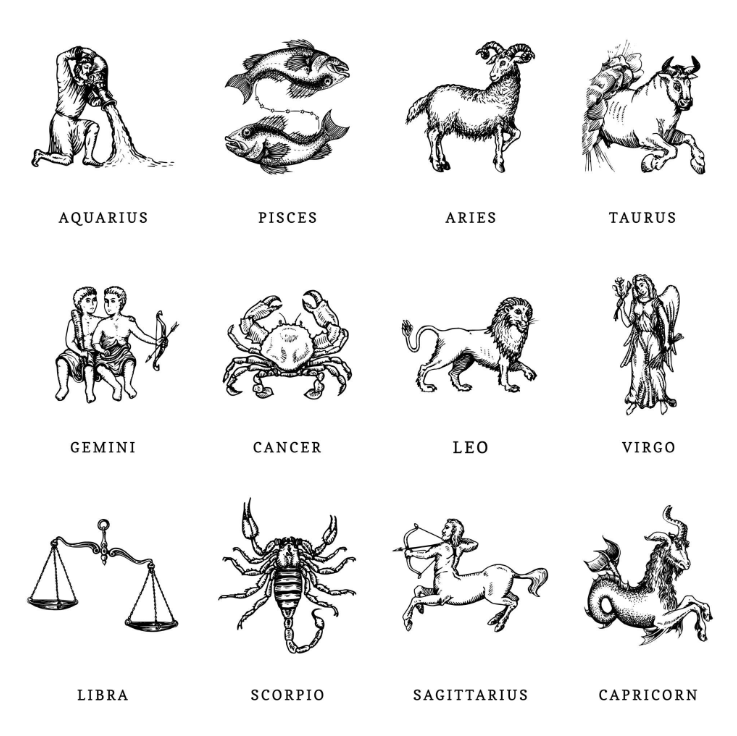
\includegraphics[scale=0.7]{Zodiac.png}
    \caption{राशी चिन्ह}
    \label{fig:sternzeichen}
\end{figure}
\subsubsection{१ -- मेष / \textenglish{Aries}}
\begin{itemize}
    \item \bt{स्वर} - अ, \bt{रंग} - रक्त (खून जैसा लाल)
    \item \bt{चिन्ह} - भेड़ (\textenglish{Ram})
    \item \bt{मालिक} -- मंगल : जल्दबाज़ी, उत्साही (जिसके प्रवाह में बहकर गलतियाँ), धैर्यहीन, साहसी, क्रोध, सरल वाणी (जैसा लगे वैसा मुँह पे), स्वातंत्र्य प्रेमी, हठी, प्रभुत्व दर्शाना, असुरक्षितता (की भावना)
    \item \bt{उच्च} -- सूर्य : त्याग, पहल कदमी, संकल्प, आत्मसम्मान, अहंकार
    \item \tamas{\bt{नीच} -- शनि : धैर्य, परिपूर्णता, देरी, सेवा, दीर्घकालिक दुख}
    \item \bt{घ.क्र} - तर्क, एकाग्रता, शुरुआत, बुद्धि, नेतृत्व, भविष्य पर ध्यान
    \item \bt{विभाजन} - १० के ३ भाग \begin{enumerate}
        \item पैर --- काम करने की क्षमता, पहल करने की तैयारी
        \item पीठ --- बोझ उठाने की क्षमता, उत्तरदायित्व
        \item सिर --- मस्तिष्क, बुद्धिमत्ता 
    \end{enumerate}
    \item \bt{जगह} - राजधानी, पहाड, कीमती धातुओं/रत्नों की खदान
\end{itemize}
\subsubsection{२ -- वृषभ / \textenglish{Taurus}}
\begin{itemize}
    \item \bt{स्वर} - आ, \bt{रंग} - श्वेत
    \item \bt{चिन्ह} - बैल
    \item \bt{मालिक} -- शुक्र : ऐश, आराम, सुन्दरता, धन (महत्वपूर्ण लगने वाली चीजें), एकत्रित किया हुआ खज़ाना, दान अनिच्छुक, अटकी हुई विचारधारा, चयन-शील
    \item \bt{उच्च} -- चन्द्र, राहु : भावुकता, खवैय्या, देखभाल/चिंता, परिवार-केंद्रित, सीमा तक शांत; फिर ज्वालामुखी
    \item \composite{\bt{नीच} -- केतु (कुछ लोग मानते है, कुछ नहीं)}
    \item \bt{घ.क्र} - परिवार, धन, वाणी, चेहरा, भोजन
    \item \bt{विभाजन} - ५ के ६ भाग \begin{enumerate}
        \item पूँछ --- शान्ति, आराम, स्वच्छता, अपवित्र चीजों का सम्बन्ध
        \item पैर --- हठी, जबरदस्ती करने वाला, बली
        \item पाचन --- कुछ भी पचाके आगे उपयोग करने की क्षमता, धैर्य
        \item ढेर --- बोझ उठाने/उत्तरदायित्व लेने की क्षमता
        \item गर्दन --- दूसरों की सहायता करने की प्रकृति
        \item सिर, सींघ --- बुद्धिमत्ता। जैसे ग्रह उस दिशा में प्रेरित \begin{itemize}
            \item \satva{शांति}, \rajas{भ्रम}, \tamas{लड़ाई}
        \end{itemize}
    \end{enumerate}
    \item \bt{जगह} - सपाट क्षेत्र, खेत, वेश्यालय, जंगल, चतुष्पद प्राणियों के क्षेत्र
\end{itemize}
\subsubsection{३ -- मिथुन / \textenglish{Gemini}}